\begin{figure}[t]
\center
    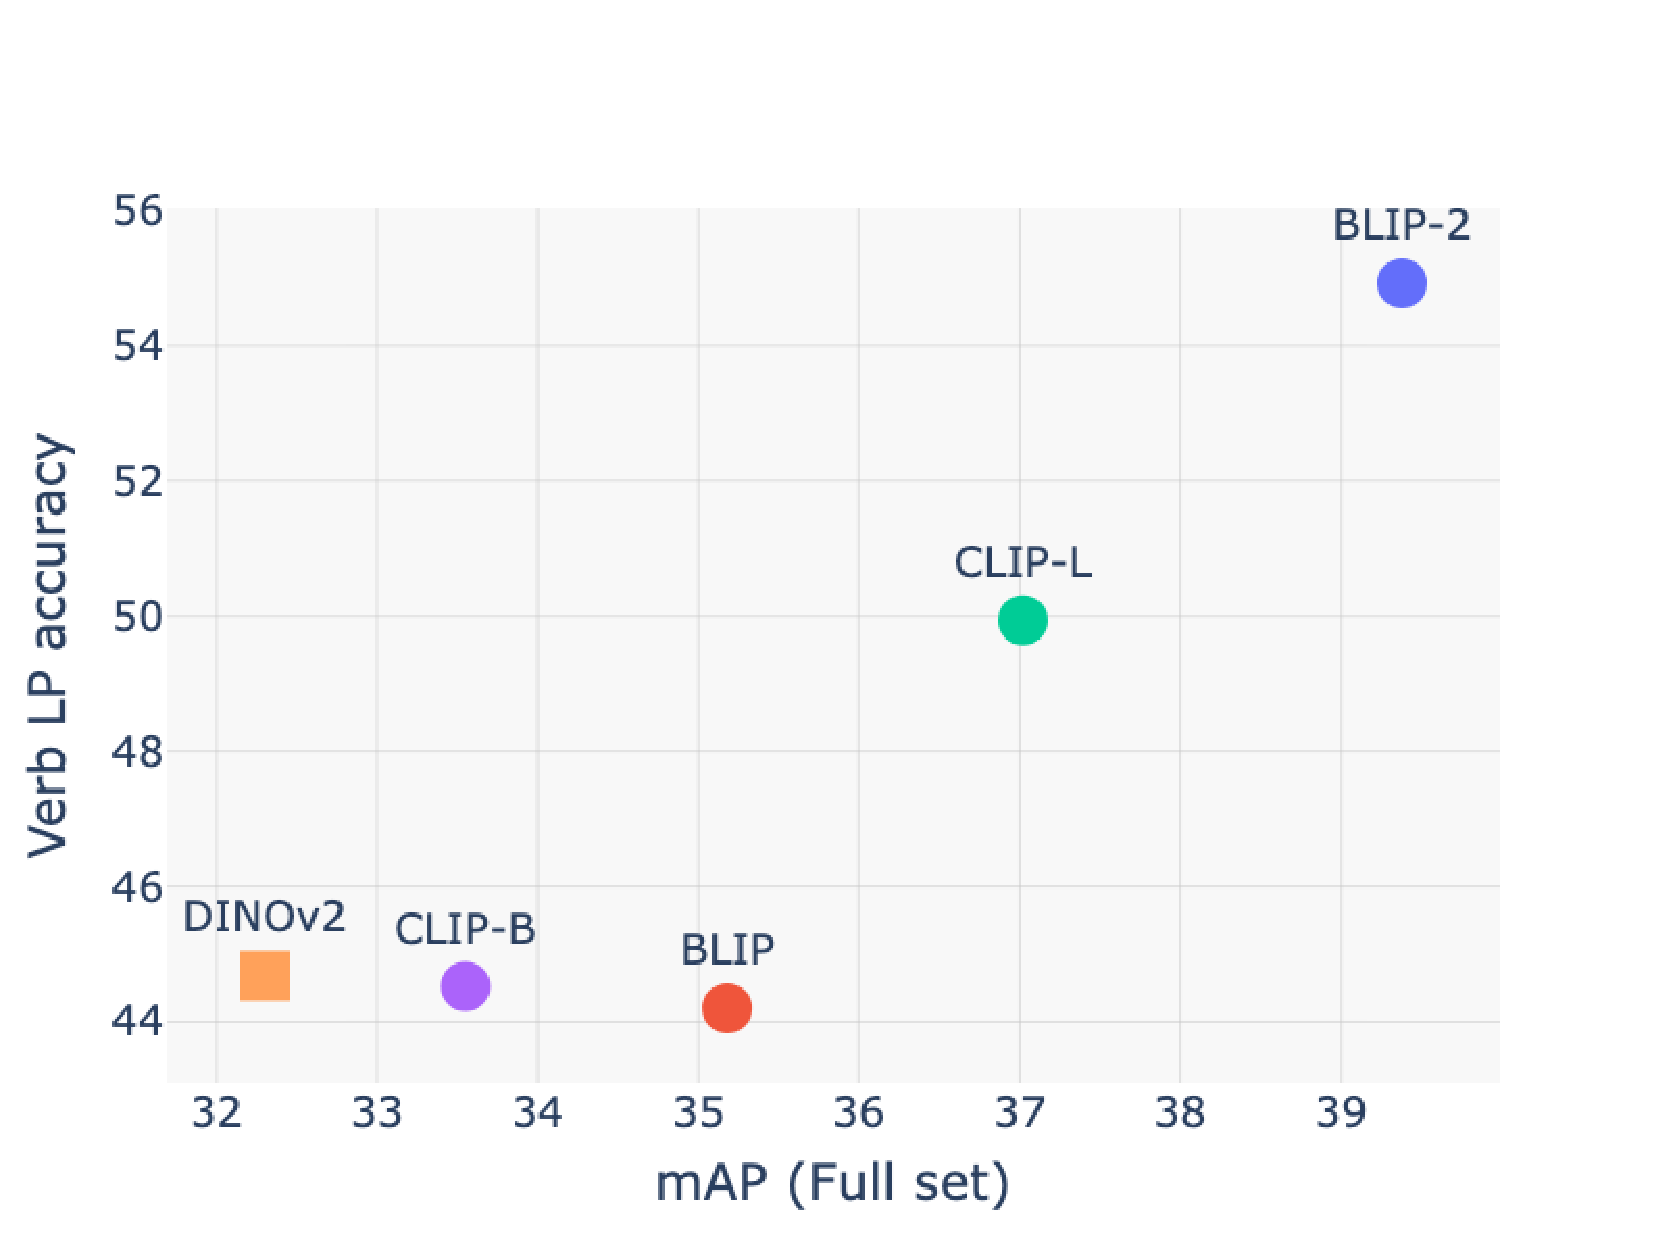
\includegraphics[width=0.5\textwidth]{figures/scatter/scat.pdf}
    \caption{
    \textbf{Dynamic Knowledge in V\&L Representations.}
    We compare linear probing results for verb prediction (LP, y-axis) and overall performance on the HOI task (x-axis) across a range of vision embeddings. We find that embeddings linearly encoding richer dynamic knowledge, as measured by the LP results, perform strongly on dynamic tasks such as HOI prediction, with the multimodal (language-supervised) embeddings of BLIP-2 achieving the best results across the board. 
    \footnotesize{Square and circular markers denote unimodal (vision-only) and V\&L-pretrained models respectively.}}
   
    \label{fig:scatter} 
\end{figure}
